%----------------------------------------------------------------------------------------
%	PACKAGES AND OTHER DOCUMENT CONFIGURATIONS
%----------------------------------------------------------------------------------------

\documentclass[twoside]{article}

\usepackage{lipsum} % Package to generate dummy text throughout this template

\usepackage[sc]{mathpazo} % Use the Palatino font
\usepackage[T1]{fontenc} % Use 8-bit encoding that has 256 glyphs
\linespread{1.05} % Line spacing - Palatino needs more space between lines
\usepackage{microtype} % Slightly tweak font spacing for aesthetics

\usepackage[hmarginratio=1:1,top=32mm,columnsep=20pt]{geometry} % Document margins
\usepackage{multicol} % Used for the two-column layout of the document
\usepackage[hang, small,labelfont=bf,up,textfont=it,up]{caption} % Custom captions under/above floats in tables or figures
\usepackage{booktabs} % Horizontal rules in tables
\usepackage{float} % Required for tables and figures in the multi-column environment - they need to be placed in specific locations with the [H] (e.g. \begin{table}[H])
\usepackage{hyperref} % For hyperlinks in the PDF

\usepackage{lettrine} % The lettrine is the first enlarged letter at the beginning of the text
\usepackage{paralist} % Used for the compactitem environment which makes bullet points with less space between them

\usepackage{abstract} % Allows abstract customization
\renewcommand{\abstractnamefont}{\normalfont\bfseries} % Set the "Abstract" text to bold
\renewcommand{\abstracttextfont}{\normalfont\small\itshape} % Set the abstract itself to small italic text

\usepackage{titlesec} % Allows customization of titles
\renewcommand\thesection{\Roman{section}} % Roman numerals for the sections
\renewcommand\thesubsection{\Roman{subsection}} % Roman numerals for subsections
\titleformat{\section}[block]{\large\scshape\centering}{\thesection.}{1em}{} % Change the look of the section titles
\titleformat{\subsection}[block]{\large}{\thesubsection.}{1em}{} % Change the look of the section titles

\usepackage{fancyhdr} % Headers and footers
\pagestyle{fancy} % All pages have headers and footers
\fancyhead{} % Blank out the default header
\fancyfoot{} % Blank out the default footer
\fancyhead[C]{ESE650 Learning in Robotics $\bullet$ March 2014 $\bullet$ Project 3} % Custom header text
\fancyfoot[RO,LE]{\thepage} % Custom footer text

\usepackage[pdftex]{graphicx}
\usepackage{epstopdf}
\usepackage{subfigure}
\usepackage{amsmath,amssymb,amsopn,amstext,amsfonts}
\usepackage{url}
\usepackage[usenames,dvipsnames]{color}
\usepackage{siunitx}
\usepackage{amsmath}
\usepackage{amsfonts}
\usepackage{amssymb}

\graphicspath{{fig/}}
\newcommand{\W}{\mathcal{W}}
\newcommand{\X}{\mathcal{X}}
\newcommand{\Y}{\mathcal{Y}}
\newcommand{\Z}{\mathcal{Z}}
\newcommand{\red}[1]{\textcolor{red}{#1}}
\newcommand{\brown}[1]{\textcolor{brown}{#1}}
%----------------------------------------------------------------------------------------
%	TITLE SECTION
%----------------------------------------------------------------------------------------

\title{\vspace{-15mm}\fontsize{24pt}{10pt}\selectfont\textbf{Gesture Recognition}} % Article title

\author{
\large
\textsc{Chao Qu}\thanks{A thank you or further information}\\[2mm] % Your name
\normalsize University of Pennsylvania \\ % Your institution
\normalsize \href{mailto:quchao@seas.upenn.edu}{quchao@seas.upenn.edu} % Your email address
\vspace{-5mm}
}
\date{}

%----------------------------------------------------------------------------------------

\usepackage{graphicx}
\begin{document}


\maketitle % Insert title

\thispagestyle{fancy} % All pages have headers and footers

%----------------------------------------------------------------------------------------
%	ABSTRACT
%----------------------------------------------------------------------------------------

%\begin{abstract}
%
%\noindent Hey, I'm just an abstract. % Dummy abstract text
%
%\end{abstract}

%----------------------------------------------------------------------------------------
%	ARTICLE CONTENTS
%----------------------------------------------------------------------------------------

%----------------------------------------------------------------------------------------
%	INTRODUCTION
%----------------------------------------------------------------------------------------

\begin{multicols}{2} % Two-column layout throughout the main article text

\section{Introduction}
\lettrine[nindent=0em,lines=2]{G}esture recognition in an interesting topic in machine learning.

%----------------------------------------------------------------------------------------
%	PRE-PROCESSING
%----------------------------------------------------------------------------------------

\section{Pre-processing}

For this project we get 9-DOF imu readings (acceleration, gyroscope and magnetometer) from a mobile phone at a sample rate of 100Hz. Although this data has been processed by the phone and has the common units, we still need to work on the data in order to use them for training and testing. The following steps are performed according to \cite{Vesa00} with some modification:

\begin{enumerate}
	\item Filter each acceleration component with fourth-order low-pass Butterworth filter with a cutoff frequency at 4Hz, see Fig.\ref{fig:imu_filt}
	\item Subsample the filtered signal at 1/5 times the original sample rate
	\item Split all the data in each gesture to a training set of 3 and valid set of 2
	\item For all the training set signal, normalize to have zero mean and unit variance and store the mean and standard deviation
	\item Cluster all training data into some number of clusters and store the centroids as our codebook, see Fig.\ref{fig:imu_cluster}
	\item Convert acceleration to sequences of observation symbols using the codebook indices
\end{enumerate}

Any new data we receive will undergo the process mentioned above and the output would be a series of observation symbols that has the same length as the data.

\begin{figure}[H]
\centering
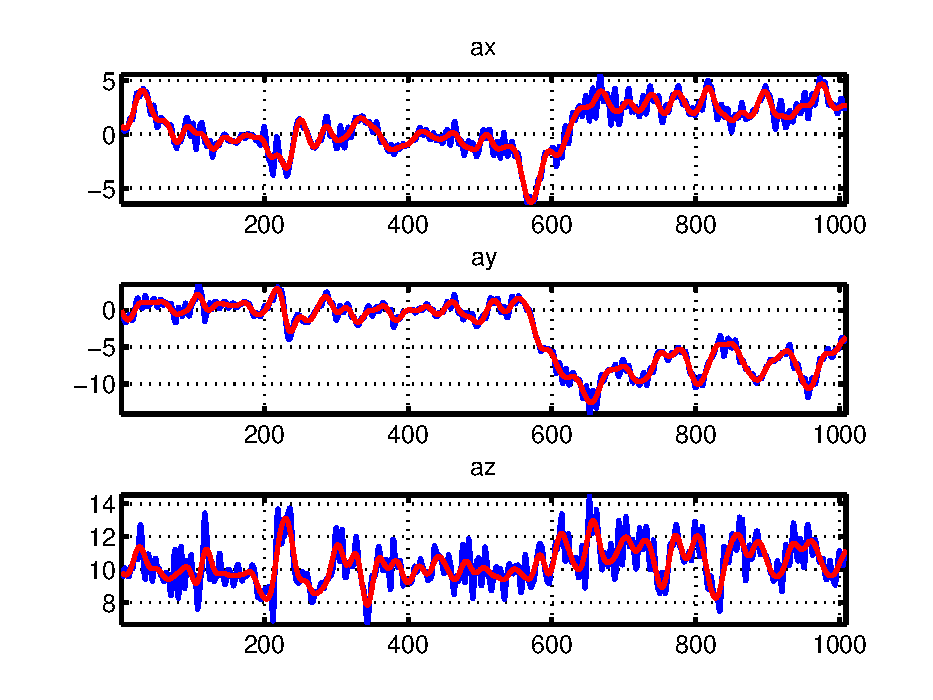
\includegraphics[width=\columnwidth]{fig/filter.pdf} 
\caption{Circle IMU data after low-pass filtering}
\label{fig:imu_filt}
\end{figure}

\begin{figure}[H]
\centering
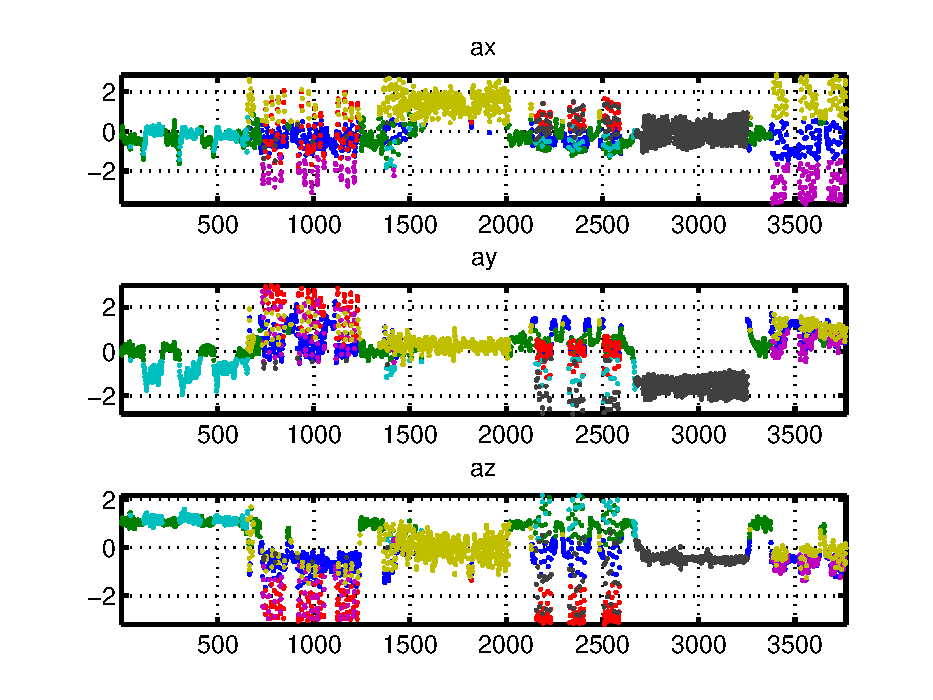
\includegraphics[width=\columnwidth]{fig/cluster.pdf} 
\caption{All training acceleration data after normalization and clustered to 7 clusters}
\label{fig:imu_cluster}
\end{figure}

%----------------------------------------------------------------------------------------
%	METHODS
%----------------------------------------------------------------------------------------

\section{Methods}
Hidden Markov model is a type of Markov process that assumes the system being modeled has unobserved hidden states. The observations are generated from the hidden states according to certain probabilities\cite{Elmez07}. A Hidden Markov model is a triple of $\lambda=(A, B, \Pi)$. 
\begin{enumerate}
	\item A set of states $Q = \{q_1, q_2, \ldots, q_N\}$ where $N$ is the number of states.
	\item An initial probability for each state $\Pi_i =\{\pi_1, \pi_2, \ldots, \pi_N\}$.
	\item An $N$-by-$N$ transition matrix $A=\{a_{ij}\}$ where $a_{ij}$ is the probability of a transition from state $q_i$ to state $q_j$, where $1 \leq i,j \leq N$. Each row of matrix $A$ must sum to $1$ for this to a probability distribution.
	\item A set of possible emission (or observation) $O=\{o_1, o_2, \ldots, o_T\}$ where $T$ is the length of the path.
	\item A set of discrete codebook symbols $V = \{v_1, v_2, \ldots, v_M\}$ where $M$ is the number of discrete symbols.
	\item An $N$-by-$M$ observation matrix $B=\{b_{im}\}$ where $b_{im}$ gives the probability of emitting symbol $v_m$ from state $q_i$. Each of of matrix $B$ also sum to $1$ to make it a probability distribution.
\end{enumerate}

The first problem we are going to solve is problem 3 in \cite{Rabiner89}, which is:

"Given an observation sequence $O$ and the dimensions $N$ and $M$, find the model parameters $\lambda=(A,B,\Pi)$ that maximizes $P(O\mid \lambda)$."

This problem can be solved using the Baum-Welch algorithm, which makes use of the forward-backward algorithm. Details of this algorithm will not be discussed here.

%----------------------------------------------------------------------------------------
%	RESULTS
%----------------------------------------------------------------------------------------

\section{Results}


%----------------------------------------------------------------------------------------
%	DISCUSSION
%----------------------------------------------------------------------------------------

\section{Discussion}


%----------------------------------------------------------------------------------------
%	REFERENCE LIST
%----------------------------------------------------------------------------------------

\begin{thebibliography}{2} % Bibliography - this is intentionally simple in this template

\bibitem{Vesa00}
Vesa-Matti Mantyla, \emph{Hand gesture recognition of a mobile device user}. Multimedia and Expo, 2000. ICME 2000. 

\bibitem{Elmez07}
Elmezain M. and Al-Hamadi A., \emph{A Hidden Markov Model-based continuous gesture recognition system for hand motion trajectory}. 19th International Conference on Pattern Recognition, ICPR 2008.

\bibitem{Rabiner89}
Lawrence R. Rabiner, \emph{A Tutorial on Hidden Markov Models and Selected Applications in Speech Recognition}. Proceedings of the IEEE, 1989.

\end{thebibliography}

%----------------------------------------------------------------------------------------

\end{multicols}

\end{document}
